\documentclass[a4paper]{article}
\usepackage[margin=1.25in]{geometry}
\usepackage{bookmark}

\usepackage{amsmath}
\usepackage{amssymb}
\allowdisplaybreaks
\newcommand\numberthis{\addtocounter{equation}{1}\tag{\theequation}}

\usepackage{mathtools}
\DeclarePairedDelimiter\ceil{\lceil}{\rceil}
\DeclarePairedDelimiter\floor{\lfloor}{\rfloor}

\usepackage{graphicx}
\usepackage{float}

\renewcommand{\baselinestretch}{1.15}
\setlength{\parindent}{0pt}

\usepackage{multirow}
\usepackage{tabularx}
\newcolumntype{L}{>{\centering\arraybackslash}X}

\usepackage[linesnumbered,ruled]{algorithm2e}
\SetArgSty{textup}

\title{{\Large CS1.305: Introduction to Algorithms Engineering} \\ \vspace{0.25\baselineskip} t-Spanner Construction}
\author{Himanshu Singh \and Pawan Karke}
\date{\today}

\begin{document}

\maketitle

\section{3-Spanner Construction}

\subsection{Algorithm}

\begin{algorithm}[H]
\caption{3-Spanner Algorithm}
\label{alg:3spanner}
\textbf{Initialization:} $E_S = R = \phi$ \\
\For{$v \in V$}{
    add $v$ to $\mathcal{R}$ with probability $\frac{1}{\sqrt{n}}$
}
\For{$v \in V - \mathcal{R}$}{
    \uIf{$v$ is not adjacent to $x \in \mathcal{R}$}{
        add all edges incident on $v$ to $E_S$
    }\Else{
        $N(v, \mathcal{R}) \leftarrow$ nearest neighbor in $\mathcal{R}$ \\
        add $(v, N(v, \mathcal{R}))$ and all lighter edges $(v, *)$ to $E_S$
    }
}
\For{$v$ belonging to a cluster}{
    \For{each adjacent cluster $c$}{
        add the least weight edge in $E(v,c)$ to $E_S$
    }
}
\end{algorithm}

\subsection{Results}

\begin{figure}[H]
    \centering
    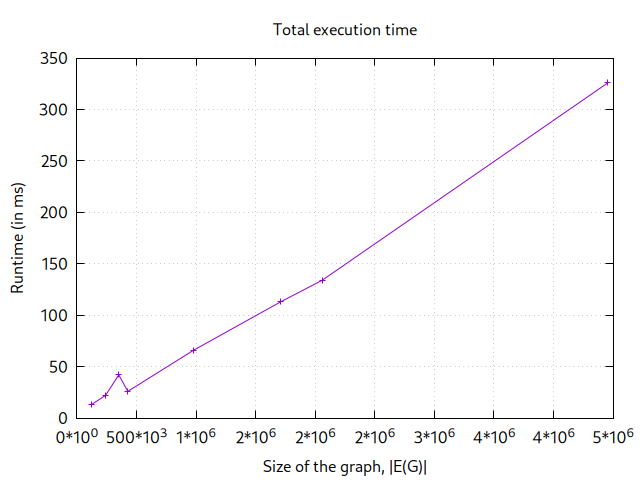
\includegraphics[width=.55\textwidth]{plots/3-spanner/execution_time.png}
    \caption{Total execution time}
\end{figure}

\begin{figure}[H]
    \centering
    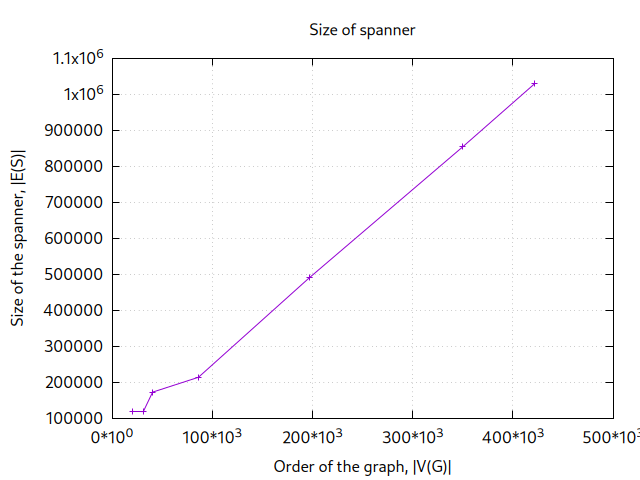
\includegraphics[width=.55\textwidth]{plots/3-spanner/spanner_size.png}
    \caption{Spanner size}
\end{figure}

\begin{figure}[H]
    \centering
    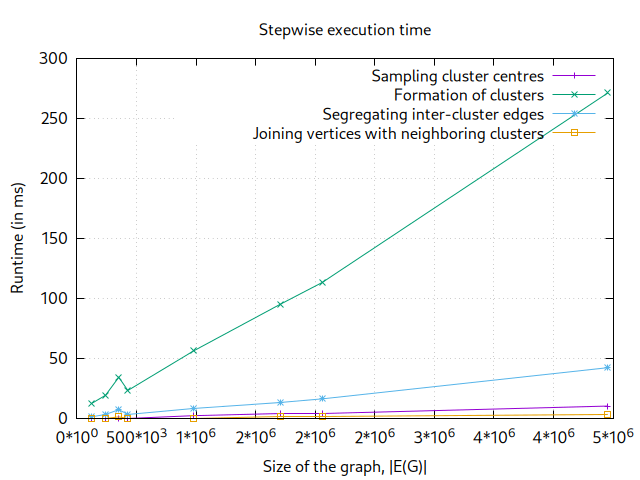
\includegraphics[width=.55\textwidth]{plots/3-spanner/stepwise_time.png}
    \caption{Stepwise execution time}
\end{figure}

\section{(2k \textminus{} 1)-Spanner Construction}

\subsection{Algorithm}

\begin{algorithm}[H]
\caption{(2k \textminus{} 1)-Spanner Algorithm: Cluster Formation}
\label{alg:cluster_formation}
\textbf{Initialization:} $E' = E, V' := V(E' \cup \mathcal{E}_{i - 1}), E_S = \mathcal{E}_0 = \phi, C_0 = \{\{v\} \mid{} v \in V\} $ \\
\For{$i \in \{1, 2, \ldots{}, num\_iterations\}$}{
    sample clusters $\mathcal{C}_i$ from $\mathcal{C}_{i - 1}$ independently with probability $n^{-\frac{1}{k}}$ \\
    \For{$v \in V' \backslash \cup \mathcal{C}_i$}{
        \uIf{$v$ is not adjacent to $c \in \mathcal{C}_i$}{
            \For{$c' \in \mathcal{C}_{i - 1}$}{
                add the least weight edge $E'(v, c')$ to $E_S$ \\
                remove the edges $E'(v, c')$ from $E'$
            }
        }\Else{
            $c, e_v \leftarrow$ nearest cluster in $\mathcal{C}_i$ and leading edge \\
            add the edge $e_v$ to $E_s$ and $\mathcal{E}_i$ \\
            remove the edges $E'(v, c)$ from $E'$ \\
            \For{$c' \in \mathcal{C}_{i - 1}$}{
                \If{$c'$ is reachable with edge lighter than $e_v$}{
                    add the least weight edge $E'(v, c')$ to $E_S$ \\
                    remove the edges $E'(v, c')$ from $E'$
                }
            }
        }
    }
    remove all intra-cluster edges of $\mathcal{C}_i$ from $E'$
}
\For{$v \in V', c \in \mathcal{C}_{k - 1}$}{
    add the least weight edge in $E'(v, c)$ to $E_S$ \\
    remove the edges $E'(v,c)$ in $E'$
}
\end{algorithm}

\begin{algorithm}[H]
\caption{(2k \textminus{} 1)-Spanner Algorithm: Vertex Cluster Joining}
\label{alg:vertex_cluster_joining}
execute cluster formation for $k - 1$ iterations \\
\For{$v \in V', c \in \mathcal{C}_{k - 1}$}{
    add the least weight edge in $E'(v, c)$ to $E_S$ \\
    remove the edges $E'(v,c)$ in $E'$
}
\end{algorithm}

\begin{algorithm}[H]
\caption{(2k \textminus{} 1)-Spanner Algorithm: Cluster Cluster Joining}
\label{alg:cluster_cluster_joining}
execute cluster formation for $\floor{\frac{k}{2}}$ iterations \\
\uIf{$k$ is odd}{
    \For{$c, c' \in \mathcal{C}_{\floor{\frac{k}{2}}}$}{
        add the least weight edge in $E'(c, c')$ to $E_S$
    }
}
\Else{
    \For{$c \in \mathcal{C}_{\floor{\frac{k}{2}}}, c' \in \mathcal{C}_{\floor{\frac{k}{2} - 1}}$}{
        add the least weight edge in $E'(c, c')$ to $E_S$
    }
}
\end{algorithm}

\subsection{Results}

\begin{figure}[H]
    \centering
    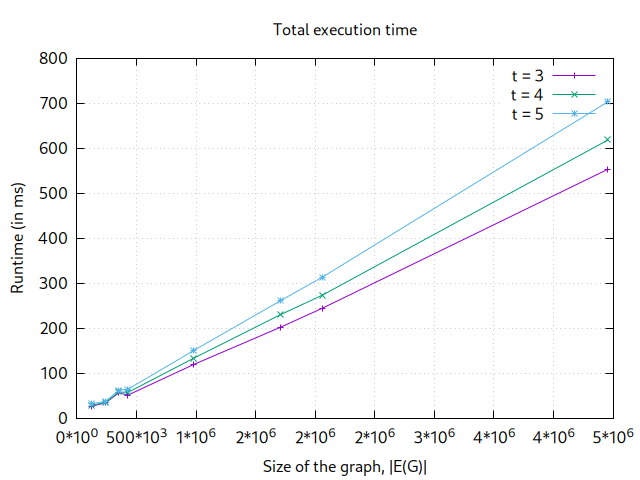
\includegraphics[width=.55\textwidth]{plots/2k-1-spanner/execution_time.png}
    \caption{Total execution time}
\end{figure}

\begin{figure}[H]
    \centering
    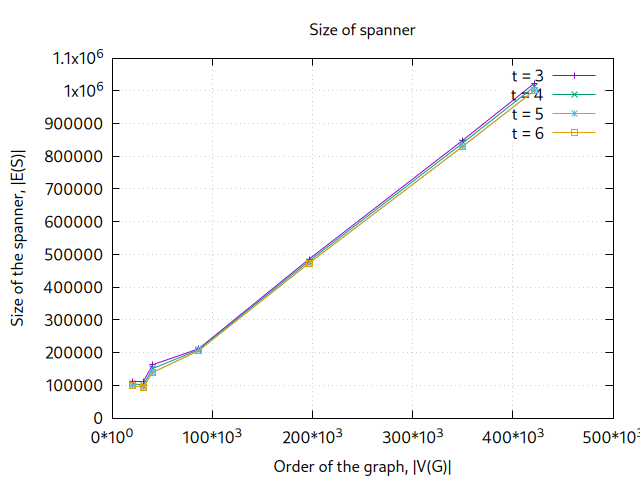
\includegraphics[width=.55\textwidth]{plots/2k-1-spanner/spanner_size.png}
    \caption{Spanner size}
\end{figure}

\begin{figure}[H]
    \centering
    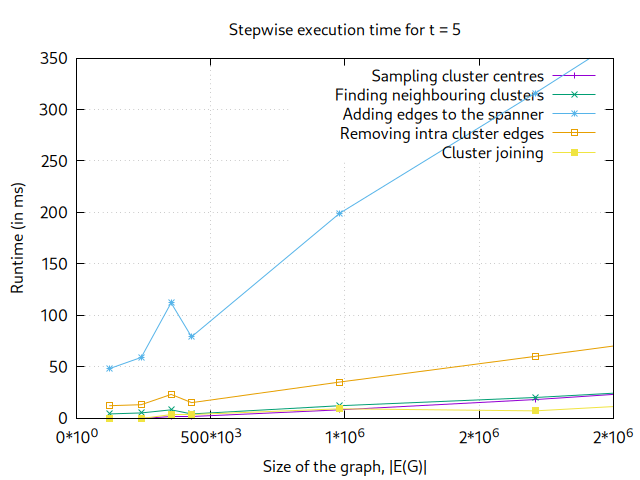
\includegraphics[width=.55\textwidth]{plots/2k-1-spanner/stepwise_time.png}
    \caption{Stepwise execution time}
\end{figure}

\section*{Bibliography}

\begin{enumerate}
\item Baswana, Surender & Sen, Sandeep. (2003). A Simple and Linear Time Randomized Algorithm for Computing Sparse Spanners in Weighted Graphs
\item Reyan Ahmed, Greg Bodwin, Faryad Darabi Sahneh, Keaton Hamm, Mohammad Javad Latifi Jebelli, Stephen Kobourov, Richard Spence (2019). Graph Spanners: A Tutorial Review.
\end{enumerate}

\end{document}
